\documentclass[11pt,a4paper,oneside]{article}

\title{\textbf{Route2Dam: Provide information on day trips to Rotterdam for students at Utrecht University}\newline \newline \newline}
\date{\today}
\author{Sorin Dragan, Evangelia Giannikou, \\Mikhail Ternyuk, Olusanmi Hundogan}
% \pagenumbering{gobble}
\pagenumbering{arabic}

\usepackage{eurosym}
\usepackage{hyperref}
\usepackage{subfig}
\usepackage{amsmath}
\usepackage{amssymb}
\usepackage{tabularx,booktabs}
\usepackage{multicol}
\usepackage{array}
\usepackage{float}
\usepackage[english]{babel}
\usepackage{quoting}
\usepackage{csquotes}
\usepackage{enumitem}
\usepackage{natbib}
\usepackage{xcolor}
\usepackage{subfiles}
\usepackage{ragged2e}
\usepackage{lmodern,textcomp}
\usepackage{graphicx}
\usepackage{titling}
\newcolumntype{M}[1]{>{\centering\arraybackslash}m{#1}}
\usepackage[backend=biber, sorting=none]{biblatex}
\usepackage[total={6.5in, 10in}]{geometry}
\addbibresource{references.bib}

\begin{document}

\maketitle


\begin{figure}[H]
    \includegraphics[width=\textwidth]{paper/imgs/Erasmusbrug_seen_from_Euromast.jpg}
    \caption{An upfront view of Rotterdam and the Erasmus bridge}
\end{figure}


\clearpage
\section{Design}
Route2Dam is an application to recommend various activities to groups on a single day trip in Rotterdam. This general goal helps to place the application in the broader taxonomy of tourism. Not only will the application deal with the type of tourism \citeauthor{dunnross_SightseeingTouristsMotivation_1991} calls 'sightseeing' but we can even place the application in a subcategory called 'city-tours'. This categorisation helps us to make assumptions about the users and the context in which they operate. The next sections will explain how the users of the system are characterized and the important contextual aspects that influences their experience. 
\subsection{User Modeling}
\label{lbl:UM}
Knowing that the application not only operates in the domain of city tours, but that the main users are students from the Utrecht university, helps creating a distinct user model for the application. In the following, we will explain who the user is, how the application adapts to the users characteristics and how the application models the users' preference. 

\subsubsection{Characterizing the individual and the group}
As mentioned earlier the goal of our application is to provide optimal guidance to groups of students visiting Rotterdam for a day trip. However, we have to rely on information of individual users to come up with a recommendation that fits the group. Hence, it is necessary to characterize the expected users of the system. In our case, the targeted user is a student of Utrecht University. Hence, we can expect a young students between 20-29 years old according to a study by \citeauthor{AgeAverage_students}. Although most students of Utrecht university being Dutch we can still assume that their different backgrounds and cultures vary significantly. This is backed up by the last Annual Report of Utrecht University (THE ANNUAL REPORT 2019) which states that 10\% of all students are non-dutch. Even among Dutch students, we can expect an increasingly diverse population of students, as early trends of the dutch \emph{Centraal Bureau voor de Statistiek} suggest.\cite{theovanmiltenburg_AllochtonenHogerOnderwijs_2007}. Students are also expected to have a relatively low average income. Although, the average income varies strongly over household types (living with parents, a student house, own house/apartment), the average of €587 remains low.\cite{kobus_OwnershipOncampusUse_2013} Hence, we can assume a high sensitivity for extracurricular expenditures. All these characteristics need to be considered, if we want to understand a users preferences. However, some dynamics only occur in groups, which is why we also have to characterize the group. We consider every set of users higher than one a group. Additionally, we assume that the users of the applications are acquainted with each other. This assumption simplifies the scope of the application in two ways. First, we do not have to introduce a person to person recommendation module. Second, we can expect communicative interactions outside of the application. However, this also introduces problems in group decision making like social confrontations and pressure. This solidifies the need for privacy and voting mechanisms within the application, if the group cannot reach a consensus.
The application will retrieve basic personal information about each user of the group via the registration process. The user’s account will store the user model, which contains a user's preferences and personal settings. The initial information  is used to create an personal set of recommendations, which can be used for solo city-trips or as part of the group's trip recommendation.
  	
\subsubsection{How do we model the users preferences?}
As mentioned earlier, the application retrieves information about the user in order to suggest a relevant guide through Rotterdam. Two major components inform our user model -- User constraints and Preference. First, a set of constraints provided by the user,


The users preferences modeling includes 2 major steps: \\	1) \textbf{Set User Constraints:}\\	
The constraints give to model general information about the user. That step is required in purpose to prepare relevant items for the pairwise comparison process at the step 2. All that information will be saved at the system, but user always can change the data provided. The constraints are following:\newline 
	- \textit{Experience}. Firstly, the users will be asked either they are first time in the city or they are local students which probably have some knowledge about Rotterdam or been there before. For the local students system will suggest more specific locations and events to choose. Also system will show places that user didn’t seen at past visits. \\
    - \textit{Budget}. The user will be asked to specify his travel budget. Nowadays, museum tickets, events or another tourist attractions can be quite expensive even with student discounts in mind. Therefore, budget constraints must be taken into account in planning.\\
  2) \textbf{Retrieving User Preferences:}\\
  The second step is the technical process of the modeling where system tries to retrieve the preferences from user without asking direct questions.\newline  
- \textit{Pairwise Comparison}. After the restrictions setting are complete for the user, the system will start the process of users preferences retrieving. The user will be asked to choose which of the two places presented by the system he wants to visit more. With each selection, the user will be provided a photo of the location and a short description of item. The minimum number of comparison rounds is 3. If the user is not satisfied with the presented locations, he can continue the selection process. As more comparisons a user uses, as more accurate the system will be able to adapt the guideline for the entire group. Actually, the weights of all members of the group are equal, but detailisation level of preferences will be higher for the user who made more choices. Hence, the probability that the system could better adapt the plan for this user will be higher.\newline
- \textit{Onsite modeling}. The group of student could not follow the complete guideline, but to choose only starting point of the possible trip. In that scenario the system calculates the time user spends in the recent location in order to suggest possible path continuation options.    
\subsubsection{How do we adapt to the user?}
Our application assumes to design an optimal list of activities for a group of students as a whole, therefore it is very important for the system to collect information about the preferences of all participants before starting the trip. Using the obtained information at the described preliminary stage, the system will design a personal rating of activities for each user. Using the previous users experience, system will choose the different items for the pairwise comparison. The user increases his chances of visiting more places of interest to him and spend an exiting day in Rotterdam. As long as system can work in 2 different ways: as a pre-planned trip or using only starting point, the application adaptation process is limited not only by the Pairwise Comparison process and settings, the system also tracks the user's movement along the designed visiting plan. When group of students choosing "starting point" regime of the trip, system gathering information along the way, like time spending at the location and suggest relevant locations as a next place to visit. Also, the user will not strictly follow the guideline all the time, and if the system determines that there are interesting sights within a 10-minute walk [.\cite{ton_CyclingWalkingDeterminants_2019}] from the current user's location and this sight might not have been included in the plan initially, the system will offer to visit it, because this will not radically change the route plan, but at the same time, the user will receive more information and impressions of the city.
\subsection{Context Model}
\label{context}
Being a recommender for city-tour activities, the application has to place a particular importance to contextual aspects of the trip. Namely, the location, the time and the weather in which the application is used. In the next paragraphs, we are going to describe how the application retrieves each contextual information and how it is used within the system to provide a contextually adaptive experience to the user.



\subsubsection{Weather}
Weather has always been an important tourism factor that requires special attention due to its unpredictable nature. Several studies a specific need for adaptation, as it is a key driver for user satisfaction or dissatisfaction.\cite{becken_ImportanceClimateWeather_2010} Among others \citeauthor{defreitas_TourismClimatologyEvaluating_2003} identifies two on-site behaviours that the application needs to take into account. Not only, do tourists want to avoid unfavorable weather conditions (eg. move from sun to shade), but they change their activity accordingly to suit them (eg. swim more/less). 

Hence, our application will retrieve weather related information about the current location from online application interfaces such as openweathermap.com. The location will be based on the longitude and latitude of the groups location. The application can use GPS coordinates from the group administrators' smartphone. We favor the geographic coordinates latitude and longitude, as they provide a more accurate retrieval of the current wheather situation, than city or regional information about the weather. In fact, a big city like Rotterdam can experience various wheather conditions in different parts of the city. 

As a result, the application will be able to filter options that are deemed unsuitable for the current weather condition. The system can, for instance, switch from outdoor activities to indoor activities and vice versa.\cite{creemers2015meteorological} This means that a park visit will not appear as an alternative during heavy rain, but indoor activities like museums or bar visits instead.

\subsubsection{Location}
The adaption to location spans two dimensions: On the one hand, we identify a static dimension as the application is adapted to the city of Rotterdam. This adaption will be covered in a later section. 

On the other hand, there is a dynamic dimension as the location of the group within the city changes constantly from activity to activity. Here, the application requires to pay special attention to spatial adaptation. The application can use GPS to locate the groups current location within the city. With this information, the application is able to adapt its recommendation in two ways. 

First, the application can provide ad-hoc recommendations for popular points of interest that are within a walking range of roughly 0.7km. We chose this heuristic based on the the maximum distance that students in the Netherlands still consider a walkable distance.\cite{ton_CyclingWalkingDeterminants_2019} This distance is equivalent to a 10min. walk, given the average walking speed of healthy individuals (4.5km/h).\cite{schimpl_AssociationWalkingSpeed_2011} As an alternative, the application could also compute the average group walking speed, but this measure might be confounded by the nature of the current visited activity or the mode of transportation. Hence, it was deemed unreliable. The "must-see"-locations will come in form of notifications which the group can choose to visit or ignore. 

The second application of location information relates to the group ranking, which will adapt based on the current location of the group. Here, the location will act as a weight for every item utility in the group recommendation list. The weighting follows the following formular.

\begin{equation}
    Utility_{i}^* = \frac{Utility_i}{\lvert Location_i - Location_G \rvert}
\end{equation}

Here, $Utility_i$ refers to the groups' utility and $Location_i$ to the location of a particular item $i$, while $Location_G$ refers to the current location of the group. This re-weighting will start after the group's completion of the first activity in the recommended list. The reason for this decision is that an earlier use of the location factor most likely leads to confusion, because it causes unexplained changes in the ranking prior to the visit [Spread of users, previsit change of ranking, XXX]. 


\subsubsection{Time \& Date}
While weather and location can be considered "soft filters", due to the groups ability to ignore these factors, the temporal context plays a crucial role for the accessibility of events, POI's or activities. As an illustration, a group cannot choose to visit a location outside of its opening hours and recommending such an item will most likely lead to strong dissatisfied responses. Hence, the applications recommendations must take temporal considerations into account. We can group these adaptation considerations based on the types of information that will be used. Namely, time (only), date (only) and time and date in conjunction. 

As the date is specified by the groups administrator upon tour creation, we do not have to resort to specific methods to retrieve the information. Similar to location, we can use the date as a notifier for upcoming events. Unlike location, the event notification will not be on-site but prior to the tour date.

The current time finds its use in discriminating between morning, daytime and nighttime activities. For that purpose we can leverage the system time of the groups administrators' smartphone. This will allow the application to favor activities suitable for the current time of the day.

The conjunction of date and time will mainly be used to filter out activities that are not accessible. Although, simple in theory, there are more additional practical considerations to take into account. First, the group must be able to reach activity on time. Second, the group should not arrive shortly before the activity closes. While the former is simple to compute, using the average walking speed of healthy individuals of 4.5km/h and the distance between the location and group, the latter highly depends on the nature of the activity. For instance, people spend approximately XX hours in a museum, while staying significantly longer in bars.\cite{MUSEUM} Furthermore, two museums can greatly differ in size, further complicating a good estimate. We chose to use the simple heuristic of 1 hour, because XXX. Resulting in the utility assignments. 
\begin{equation}
    \forall i \in O: T_i - (T_{now} + \frac{\lvert Location_i - Location_G \rvert}{4.5}) < 1 \Rightarrow Utility_i := 0
\end{equation}
$T_i$ refers to the closing time of activity $i$ in the set of all activities $O$. $T_{now}$ refers to the current time. Like with location, this update only occurs after visiting the first activity. 

\subsubsection{Rotterdam}
The last context, which is often overlooked, is the  adaption to the former European cultural capital Rotterdam.\cite{hitters_SocialPoliticalConstruction_2000} After its destruction in WW2, Rotterdam's tourism primarily focused on modern culture.\cite{rotterdam} The result of that was a modernistic architecture, which shifts away from the traditional Dutch model. The application's adaption to Rotterdam is an inherent part of design goals with regard to visuals and content. First, the application's name \emph{Route2Dam} is a word play, as it bears auditory resemblence to \emph{Rotterdam}. In terms of content, application assumes that the students will not change the location during the day trip which is why the application only shows locations and events confined to Rotterdam. Other locations are excluded. The user interface (UI) of the application was created with Rotterdam's modernistic architectural design in mind. An example of this can be seen in the splash screen, which shows the Erasmus bridges' silhouette. However, more details about visual design decisions are going to be elaborated in the UI section of this paper.

\subsection{Adaptive Hypermedia}
The adaptive hypermedia part of the system revolves around the pairwise comparison. Our system will show each user a different items to compare depending on his selection. This procedure resembles the way other adaptive hypermedia systems show different content depending on the order of the links that have been clicked. Hence, this section will how items are presented towards the user and how they are initially chosen. 

\subsubsection{Presentation of Pairwise Comparisons}
As mentioned in \autoref{lbl:UM}, this system will use a series of pairwise comparisons to model the preferences of a user. These pairwise comparisons are presented in the form of two items being shown on a screen. It has long been known that users find choosing between two items easier than choosing among a set of options.\cite{COGNITIVE_OVERLOAD} The user will then be able to click on either of the items. Clicking an item is equivalent to stating that the clicked item is preferred over the alternative. Subsequently, the user will have to answer the next pairwise comparison query. This querying process repeats at least three times. Afterwards the user is free to either compare more items or to end the process.

There are two alternatives to the approach of showing the next queries: Either letting the unpreferred activity vanish instead of the preferred item or letting the user choose among two completely new items. 

The last option may provide the opportunity to explore the latent preference function more as we can sample items from different parts of the items space. However, unlike with the former alternatives we cannot leverage a crucial advantage of preference relations -- the transitivity of preference alternatives.

The rule states, that if item a is preferred over item b and item b is preferred over item c, then under the assumption of preference consistency the user also prefers item a over c. Meaning, that we attain three pairwise comparison results from asking two pairwise comparison queries. However, this approach also comes with problems, due to its consistency assumption. We cannot always assume that the user will answer consistently.

The application will employ the latter option, as it allows to exploit transitivity to gain more knowledge about the user. Although consistency being a strong and unlikely assumption, the probablistic nature of the pairwise-comparison model mitigates the uncertainty arising from inconsistent query responses.


\subsubsection{Query Pair Selection}
\label{sec:pair}
Now that we have explained how the queries are selected two questions remain: How do we select the individual pairs and how can we use the query results to recommend an ordered list of activities. In this section, we will answer the former question, while the latter will be answered in \autoref{sec:rs}. 

As mentioned prior, the application needs to select different pairs of items based on his former query responses. Given that we do not know anything about the user's preferences at the beginning, we first have to explore the space of possible preferences as much as possible. The application achieves this by asking by querying pairs that are diametrically opposed. Starting with a randomly selected activity, the application chooses another activity, that maximizes the dissimilarity between both activities. As every activity is represented as vector, we can use any vector similarity metric such as the cosine similarity or any Minkovski distance (e.g.: Euclidian distance). However, after the first query result, we cannot rely on this method anymore, as the next maximally dissimilar item would be very similar to the item that vanished after the first decision. In other words, we need to query for an item that is maximally dissimilar to the first pair. For that purpose, we can find the activity that is the most similar to the cross product of both activity vectors. Mathematically the cross-product of two vectors yields a vector that is linearly independent from both initial vectors. In other words, the cross-product has a 90° degree angle to the plane that both vectors form and is maximally dissimilar to both if we consider the angle as measure for similarity. As a result, we will apply cosine similarity consistently as similarity measure for all activities as it uses the angle between vectors. \autoref{fig:item_vectors} illustrates the above reasoning. Now, that we've explained the decision for the first two query pairings, we can now repeat the established process. 

\begin{figure}[H]
    \centering
    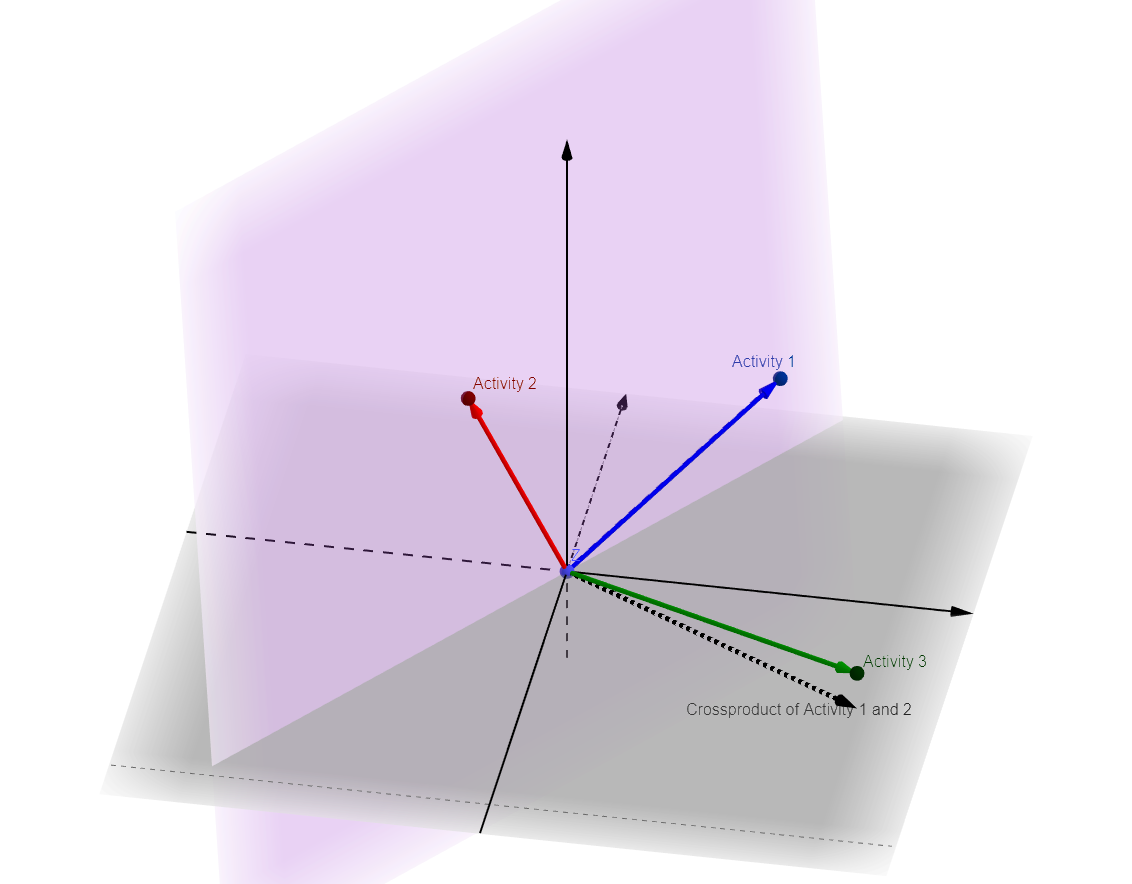
\includegraphics[width=0.75\textwidth]{paper/imgs/geogebra-export.png}
    \caption{Image shows three activities (red, blue, green) represented as vectors. The red activity and the blue are dissimilar as their angle is large. Both vectors span a plane, whose normal vector we can compute with the cross product. We can find the next activity by finding the activity whose angle is closest to the cross product. In this example, that would apply to the third activity (green)}
    \label{fig:item_vectors}
\end{figure}

This approach is viable for exploring multiple opposing angles of preferences. However, as mentioned above, we also have to elicit the intricacies between activities that are roughly similar but differ in detail. A user might like going to museums, but may prefer a contemporary arts museum over a natural history museum. The simplest solution is to alternating the aforementioned procedure with one that picks a similar activity as next query partner. As stated before, we start with the alternation after the third query response. 
In figure \autoref{fig:pairing_process}, we show the full process.

\section{Recommender System}
\label{sec:rs}
The recommender system will provide the users a way to settle on an common itinerary for a day trip to Rotterdam. The system will achieve its goal by taking into account concepts as privacy, social pressure, and cognitive overload [maybe cite]. The users interact with the system through an application installed in their personal phones. By having the application on the phone, the users can decide independently about their preferences and expectations regarding the trip. In this manner, we guaranty privacy and avoidance of social pressure. As the system is a group recommendation system, we use an egalitarian approach to aggregate the preferences and generate the group recommendations. When aggregating, this is done by attributing the same weight to each individual ranking and not balancing by taking into account the number of queries to which each user responded.

The recommender system can be thought of as a pipeline of 3 independent components. The first component (\textbf{Individual User Recommendations Component}) will take the preferences of a user and convert them into a personal ranking of possible activities. This is achieved by framing the problem as a preference elicitation problem with a focus on using pair wise comparisons. Having generated the individual rankings for all the members of a group, the second component (\textbf{Ranking Aggregation Component}) will then aggregate the rankings into a group ranking of possible activities. At this point, the users will choose an item from the ranking and the third component (\textbf{Routing Component}) will use route recommendation techniques to guide the group towards the location of the chosen activity. Outside of the 3 components, a set of \textbf{preliminary filters} will be applied to the activities before entering the pipeline. Each component will be discussed in detail in the following subsections.

\begin{figure}[H]
    \centering
    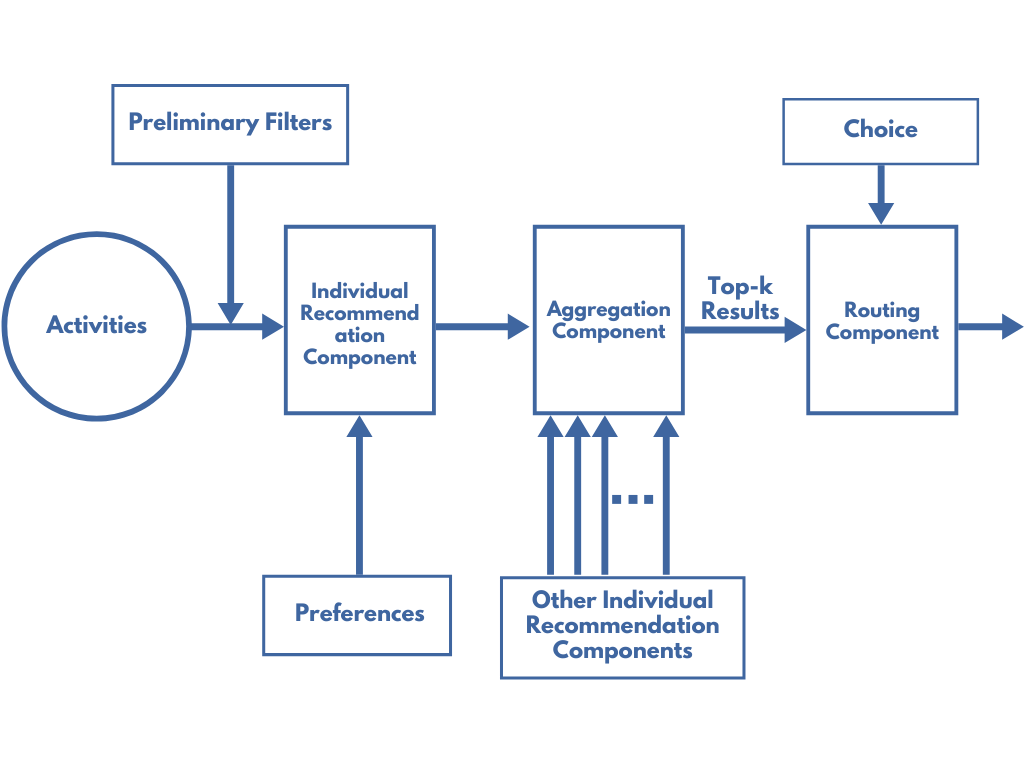
\includegraphics[width=0.8\textwidth]{paper/imgs/chart_ais.png}
    \caption{The simplified pipeline including the main components of the Recommender System described in this section}
    \label{fig:pipeline}
\end{figure}

\subsection{Preliminary Filters}
The system discards some activities from the list by considering some preliminary filters. Examples of such filters are being Dutch or International, the maximum budget set by the user, the start hour of the trip etc. These preliminary filters are backed up by simple assumptions that might improve the overall experience. If all the group members are international, it does not make sense for the system to include cinemas where the movies are in Dutch without an English subtitle. It also benefits to exclude activities in location that are closed before the start time of the trip or that are to expensive for the overall budget of the user. Applying these filters will remove inconsistent activities and therefore will simplify the recommendation process.

\subsection{Individual User Recommendations}
The systems has access to a vast list of activities that can be done in Rotterdam. The goal of the Individual User Recommendation component is to sort this list according to the user's preferences, thus creating a desirable ranking of activities. The ranking will be generated using pairwise comparisons, or \textbf{queries}. In the case of our system, a query is represented by presenting two specific activities to the users from which they will choose the one that suits them the most, thus eliminating the other. From this choice, a order can be inferred for the two alternatives; activity $i$ is preferred over activity $j$: $q_{i,j} = a_i < a_j$. As we do not have access to enough queries ($n\cdot log(n)$, where $n$ is the number of activities in the list) to sort the list and considering the fact that any preference ranking can be equated by an utility function defined on the domain of preferences, we will make use of introduced uncertainty and treat the problem as a \textbf{preference elicitation problem}. We will use the Gaussian Process Preference Elicitation approach described by Guo et al. [cite here] to derive the result of new queries without the user's input. Our choice is supported by the non-parametric Bayesian nature of Gaussian Processes which translates in having a flexible model of user's utility. The model works under uncertainty and can easily integrate new information. The model also proves to be more efficient than a classical content/user filtering recommender system which assumes a large user-base. Additionally, the inner workings of the system can automatically handle the cold-start problem present in other recommender systems.

In this approach, both the users and activities are represented by feature vectors. This facilitates the use of similarity metrics both between items, and between users. By doing so, we can easily offer a solution of the cold start problem in recommender systems. When a new user enters the system, the systems will use the hard filters, the result of the queries and a taxonomy of activities to construct the feature vector of the user. The hard filters can be used directly in constructing some useful features. If the user is international, has never been to Rotterdam before, and has a budget of \EUR{60}, a vector covering this 3 dimensions can have the following form: $[1, 0, 60]$. In the case of the queries, a simple inference using the defined taxonomy is necessary to construct other features. If the user prefers going to the "Museumpark" instead of going to "LantarenVenster", we can make the assumption that the user enjoys Parks (the superclass of every park), but does not enjoy Cinemas (the superclass of every movie theater). Therefore, we mark Parks with a $1$ and Cinemas with a $0$ in the feature vector representing the user. Having each user represented by a vector allows using, alongside the user's query responses, the similarity with other users for which we have more information, thus resulting in a faster generation of individual ranking.

As mentioned above, we will model the utility function using a Gaussian Process having the following form:
\begin{equation}
    \label{gp}
    f(u, a) \sim GP(0, k^u(u,u')k^a(a, a'))
\end{equation}
$a$ and $a'$ are two different activities. Same holds for $u$ and $u'$ as two distinct users. $k^u$ and $k^a$ are the covariance functions on the user feature vectors and, respectively, the activity feature vectors. Each covariance function, or \textbf{kernel}, comes with its own hyperparameters ($\theta$) used in regression settings.

We assume the users' preferences to be conditionally independent as we consider the theoretical best-case scenario in which the users will not be influenced by external parties in stating their personal preferences and self-applied restrictions, thus avoiding social pressure and group bias. Under this assumption the we model the probability of a user $u$ to prefer an activity $a$ over $a'$ as shown in equation \ref{eqm}, where $f$ is the previously mentioned utility function.
\begin{equation}
    \label{eqm}
    p(a^u > a'^u | f(u,a) - f(u,a'), \xi) = I[\xi \leq f(u,a) - f(u,a')]
\end{equation}
Here, $\xi$ is a normally distributed variable which guides the value of $f$ such that the stated relation holds. $I$ has value $1$ if $\xi \leq f(u,a) - f(u,a')$ is true and $0$ otherwise. Following the paper, from \ref{eqm}, we can deduce the respective normal cumulative distribution function and the probability of having some observations given the utility function $f$:
\begin{equation}
    \label{eqm}
    p(O|f) = \prod_i^U \prod_{j, j'}^A \frac{1}{\sigma} (f(u^i, a^i_j) - f(u^i, a^i_{j'})) 
\end{equation}
where $U$ is the set of users, $A$ is the set of activities and $\sigma$ is the standard deviation of $\xi$. 

Now we can model the posterior and predictive distributions using the Bayesian Inference formula in equation \ref{bayes}, where $f$ is again the utility function, $O$ are the observed query results, and $\theta$ stands for the kernel hyperparameters.
\begin{equation}
    \label{bayes}
    p(f|O, \theta) = \frac{p(O|f,\theta) \cdot p(f|\theta)}{p(O|\theta)} 
\end{equation}
Equations \ref{posterior} and \ref{predictive} show the resulted posterior and predictive distributions. The posterior distribution was calculated by a Laplace approximation followed by an iterative application of the Newton's method to derive the maximum posterior $f_{max}$. The predictive distribution from \ref{predictive} will be use to elicit the preferences of an user $u^*$ over two unseen activities $a^*_1$ and $a^*_2$. 
\begin{equation}
    \label{posterior}
    p(f|O) = N(f|f_{max}, (W + \Sigma^{-1})^{-1})
\end{equation}
\begin{equation}
     \Sigma = K^u \otimes K^a
\end{equation}
where $\otimes$ is the Kronecker product between the covariance between all the user vectors $K^u$ and the covariance between all the activities vectors $K^a$; $W$ is the ratio between the function and the first derivative of the function present in Newton's method iterative approach.
\begin{subequations}
\label{eqn:preddist}
\begin{equation}
    \label{predictive}
    p(f^*|O) = N(f^*|\mu^*, C^*)
\end{equation}
\begin{equation}
    \mu^* = (k^*)^T\Sigma^{-1}f_{max}
\end{equation}
\begin{equation}
    C^* = \Sigma^* - (k^*)^T(\Sigma - W^{-1})^{-1}k^*    
\end{equation}
\end{subequations}

\autoref{eqn:preddist} shows that we only have to compute $\mu^*$ to get an estimate for the unknown values in $f^*$. The computed covariance $C^*$ is not necessarily required for the application but it provides us with the level of uncertainty for the estimation.
 
\begin{subequations}
    \label{eqn:computation}
    \begin{equation}
         k^* = (k^*)^u \otimes (k^*)^a
    \end{equation}
    \begin{equation}
         (k^*)^u = [k^u(u^*, u_1),\hspace{5} ...\hspace{5} k^u(u^*, u_{|U|})]
    \end{equation}
    \begin{equation}
         (k^*)^a = \begin{bmatrix}
       k^a(a^*_1, a_1),  \hspace{5}...\hspace{5}  k^a(a^*_1, a_{|A|}) \\
       k^a(a^*_2, a_1),  \hspace{5}...\hspace{5}  k^a(a^*_2, a_{|A|})
       \end{bmatrix}
    \end{equation}
    \begin{equation}
         \Sigma^* = \begin{bmatrix}
       k^u(u^*,u^*)k^x(a^*_1, a^*_1) &
       k^u(u^*,u^*)k^x(a^*_1, a^*_2) \\
       k^u(u^*,u^*)k^x(a^*_2, a^*_1) &
       k^u(u^*,u^*)k^x(a^*_2, a^*_2) 
       \end{bmatrix}
    \end{equation}
\end{subequations}
We can use the described process to find the most k preferred activities for every user. Hence, we also provide individual recommendations, even if the macro system is defined for group recommendations. 

As a last mention, naturally, we would try to a achieve sufficiently good ranking with as few queries as possible. The first queries will contain very dissimilar activities, as they carry much more information, but gradually, if the user keeps choosing, more similar activities will also appear in the queries. Hence, with more information, the resulting ordering of the activities will be closer and closer to the optimal one, assuming at least one optimal ordering exists for a specific user. The procedure of choosing the queries was elegantly described in section \ref{sec:pair}.

\subsection{Ranking Aggregation}
Having obtained the rankings for all the users we will we need a method to easily aggregate them into a group ranking. Here we will make use of the game theoretic notion of social choice. More specifically, we will use Borda voting [cite MAS book]. Borda voting functions by taking the fully ordered list of preferences of each user and assigning points in descending order from the top preference to the lowest-ranked preference. This can be further illustrated by a simplified example. 
Assume we have a group of 3 users \{$u_1$, $u_2$, $u_3$\} and 4 possible activities (after filtering) \{$a_1$, $a_2$, $a_3$, $a_4$\}. Consider the following resulted individual rankings: $u_1$ : $a_1 > a_2 > a_3 > a_4$, $u_2$ : $a_3 > a_2 > a_1 > a_4$, and $u_3$ : $a_2 > a_3 > a_4 > a_1$. This will translate to the following Borda voting vectors: \\
\begin{center}
    \begin{matrix}
    A \\
    a_1: \\
    a_2: \\
    a_3: \\
    a_4: \\
    \end{matrix}
    \begin{matrix}
    u_1 \\
    3 \\
    2 \\
    1 \\
    0 \\
    \end{matrix}
    \begin{matrix}
    u_2 \\
    1 \\
    2 \\
    3 \\
    0 \\
    \end{matrix}
    \begin{matrix}
    u_3 \\
    0 \\
    3 \\
    2 \\
    1 \\
    \end{matrix}  
\end{center}

From here, we can obtain the group ranking by adding the vectors together:

\begin{equation}
    \begin{bmatrix}
    3 \\
    2 \\
    1 \\
    0 \\
    \end{bmatrix} + 
    \begin{bmatrix}
    1 \\
    2 \\
    3 \\
    0 \\
    \end{bmatrix} + 
    \begin{bmatrix}
    0 \\
    3 \\
    2 \\
    1 \\
    \end{bmatrix} = 
    \begin{bmatrix}
    4 \\
    7 \\
    6 \\
    1 \\
    \end{bmatrix}
\end{equation}
This vector now translates back to the group ranking of activities $a_2 > a_3 > a_1 > a_4$.

We use Borda voting as we have direct access to the sorted list of each group member as soon as the execution of the first pipeline component is ready. Another reason to use Borda voting lays in the fact that it provides a very fast preference aggregation in the form of adding $|U|$ ($U$ is the set of users) vectors which can be done in $O(1)$ time. Because all the necessary operations are vector additions, the input of the aggregation component does not introduce a computational bottleneck. The vectors can be added in any order and there is no need in pausing the execution in order to collect the resulted data from all the users.

\subsection{Routing}
Two possible scenarios are possible after the computation of the group aggregate ranking of activities: creating a \textbf{visiting plan} including all the recommendations in the top-k ranking or choosing a \textbf{first destination} on which the group agrees. Both scenarios will be further described next, in reverse order.

Section \ref{context} already described an online adaptation based on location, distance, and budget. However, this adaptation begins after the first activity was finished. Being presented with the top-k ranking, the group must decide on the starting activity. This can be done by in person negotiation and argumentation. Even so, it can happen that the group is unable to reach an unanimous decision or several people refuse to take part in the negotiation. For these reasons, we propose a simple solution. The group will be presented with a new voting round. Both plurality voting and approval voting [cite MAS book] are good candidates for this scenario. After computing the winner of the vote, each member of the group will be redirected to their default Maps application in which a route to the location of the desired activity will be presented. After having finished the first activity, the ranked list of activities will be shifted upwards. As the adaptation techniques described in section \ref{context} work with real values, rather than ordered list, the list will be min-max normalized such that any position in the list will have an utility between $0$ and $1$.

The second scenario translates in a visiting plan tailored for the day trip. If the members of the group are happy with all the top-k recommendations, the system can create a route that includes all of them. Each activity will be treated as a node in a complete weighted directed graph. A dummy start node that has only out edges will also be added. The weight of each incoming edge to a node will be a combination between the geographical distance between source node and the destination node, the average time spent in the destination node, and the expenses attributed to the activity represented by that node. To arrive at a formula for computing the weights based on previously mentioned 3 arguments, a couple of assumption will be made. A minimum geographical distance to the activity is desirable. Lower expenses are desirable over higher expenses. Even more precisely, lower expenses for an activity which can be enjoyed longer is preferred over higher expenses for an activity that has a shorter time frame. This assumptions have been summarized in formula \ref{weights}.
\begin{equation}
    \label{weights}
    w = d + m \cdot (1 - t)
\end{equation}
Several things must be mentioned here. Firstly, $w$ stands for the weight, $d$ is the geographical distance, $t$ is the time frame, whilst $m$ represents the amount of money. Secondly, all the values that enter the formula have been min-max normalized in advanced, thus we deal only with values in the $[0, 1]$ interval. Lastly, as we model this as a shortest path problem, the lower the weight, the better. At this point we have constructed the graph. Evidently, calculating a path through all the activity nodes, without visiting two nodes twice happens to be the well-studied \textbf{Travelling Salesman Problem}(TSP) from computer science. We deal with an NP-hard problem that where a solution can be achieved, without stochastic using stochastic methods, with the worst-case time complexity of $O(2^nn^2)$ and space complexity of $O(2^nn)$. However, we must remember that we area dealing with a graph with $k+1$ nodes, where k is a very small number (a one digit number). This implies that we can solve the problem using the Held-Karp algorithm, thus providing a well-adjusted visiting plan for the group.

\section{User Experience}
Route2Dam is a modern designed mobile application aiming to attract users of a young age. The design of it is simplistic, with elements that adapt to the environment of the application. As previously mentioned, the name is a wordplay for Rotterdam, easy to remember, and accurate, as it gives out what the concept of the application is. In addition, inspired by the fact that water is an integral element of the city, Rotterdam is the largest port in Europe, the primary color of the user interface is blue. Finally, the splash screen shown in figure \ref{fig:splash_screen} is an example of a design adaptation that illustrates a figure of the Erasmus bridge, one of the most important landmarks of the city. To combine it with the overall Dutch identity, the colors of the name were based on the Dutch flag. 


\begin{figure}[H]
    \centering
    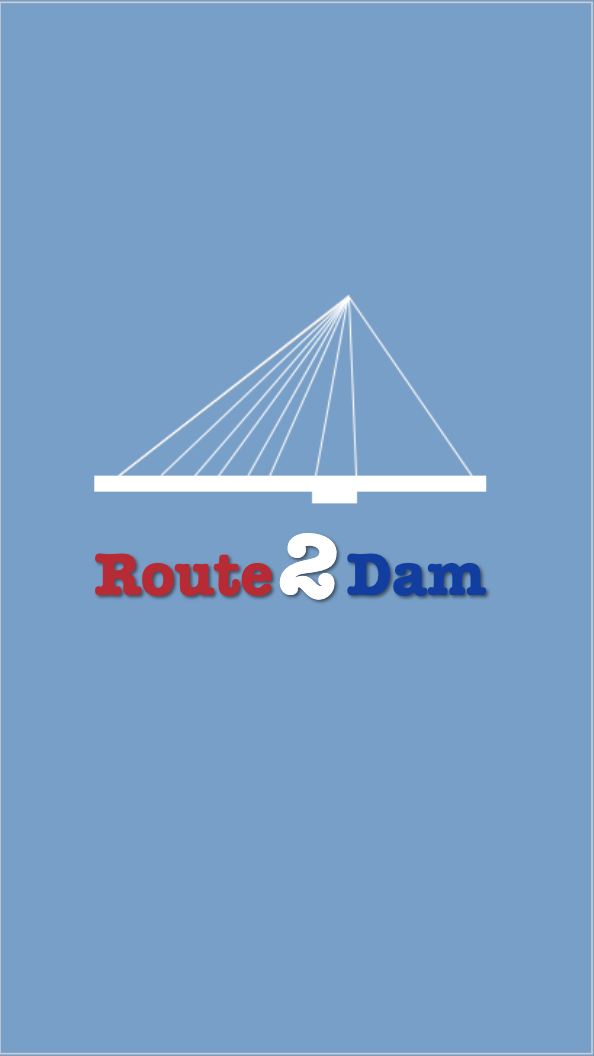
\includegraphics[width=0.3\textwidth]{paper/imgs/hifi_prototypes/splash_screen.png}
    \caption{The splash screen of Route2Dam}
    \label{fig:splash_screen}
\end{figure}

The application has two types of users; the administrator and the simple users. Both types need to set up their personal and trip settings and can pick the activities they would like to do. 

The administrator is considered the person to first create a new trip on the application, and he is distinguished by a small “crown” icon. His additional feature is that he can invite his friends (simple users) to join the application but also set a starting point for the trip. The simple user's feature is accepting or rejecting the administrator’s proposals.

Initially, the administrator is starting a new trip and sets up his profile and trip preferences. As shown in figure \ref{fig:profile_trip_settings}, these involve his name, if he is Dutch or no, and if he has been before to Rotterdam. Also, he needs to set an approximate amount of money he is willing to spend so that the application does not show results that are over the group’s budget. In the trip settings, the timeframe of the day trip is set to show only activities and places that are open during the visit.

\begin{figure}[H]
    \centering
    \subfloat[\centering]{{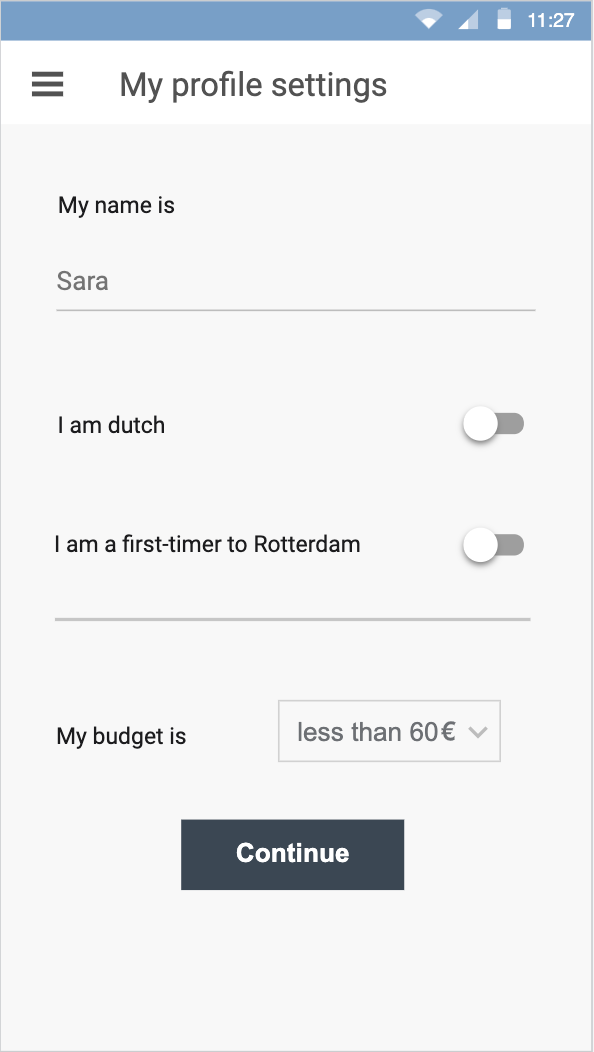
\includegraphics[width=0.3\textwidth]{paper/imgs/hifi_prototypes/profile.png} }}%
    \qquad
    \subfloat[\centering]{{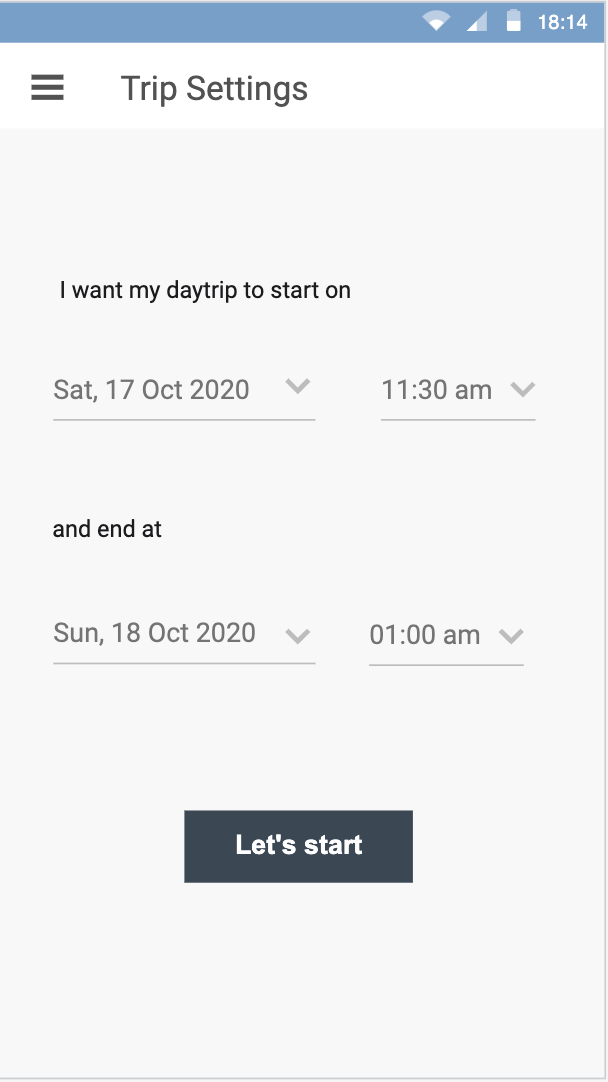
\includegraphics[width=0.3\textwidth]{paper/imgs/hifi_prototypes/trip_settings.png} }}%
    \caption{The profile and trip settings screens }%
    \label{fig:profile_trip_settings}%
\end{figure}

Afterward, the administrator can send an invitation to other users by clicking on the "add" button at the bottom of the left navigation drawer as shown in figure \ref{fig:left_menu}. The button triggers an invitation link sent through other messenger applications (WhatsApp, Messenger etc).

\begin{figure}[H]
    \centering
    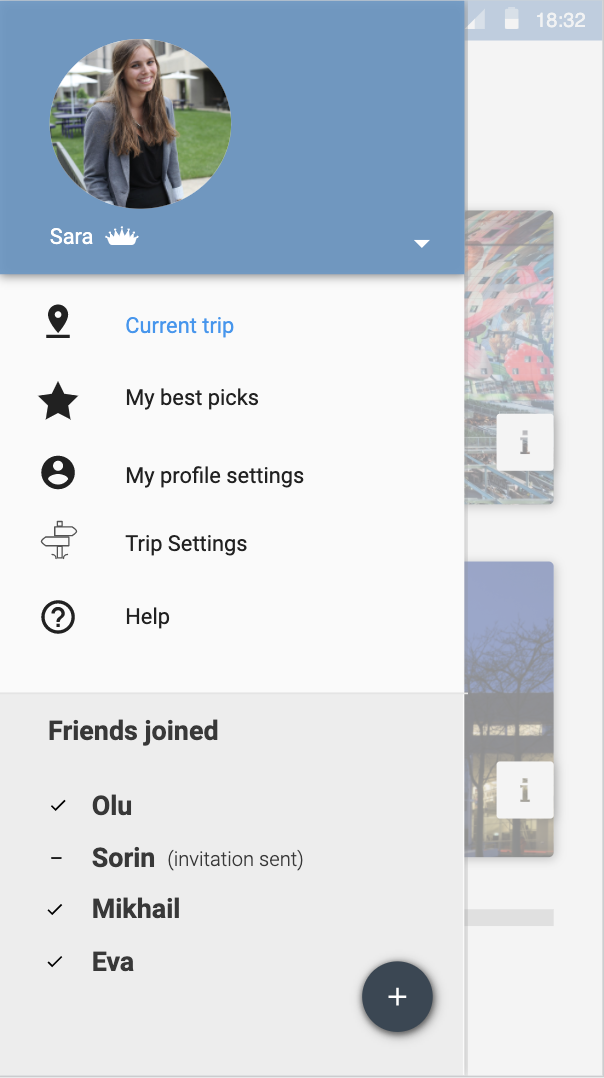
\includegraphics[width=0.3\textwidth]{paper/imgs/hifi_prototypes/left_menu.png}
    \caption{The left navigation drawer}
    \label{fig:left_menu}
\end{figure}

Apart from the invitation button, this screen is also available for simple users, so both user types share the same user interface. Once the user has set up his personal preferences, the data are stored in the application and are accessible from the left navigation drawer. For example, his personalized suggested activities are available under the “My best picks” item. The reason is that next time he uses it for another trip, he will not have to reset his preferences and will “save” some time. Another feature of this screen is that everyone can see who has already joined the account or even upload a profile picture.

Assuming that both the administrator and the other users have “joined” the trip account and set up their initial settings, they are all prompted to the pairwise comparison screen as in figure \ref{fig:pairwise_comparison_screens}.

There, the user gets two different options, and by clicking on one of the images, he moves on to the next pair for a minimum of 3 times. At last, the system urges the user to either continue the customization and move to another round of pair comparisons or show him some suggested activities.

\begin{figure}[H]
    \centering
    \subfloat[\centering]{{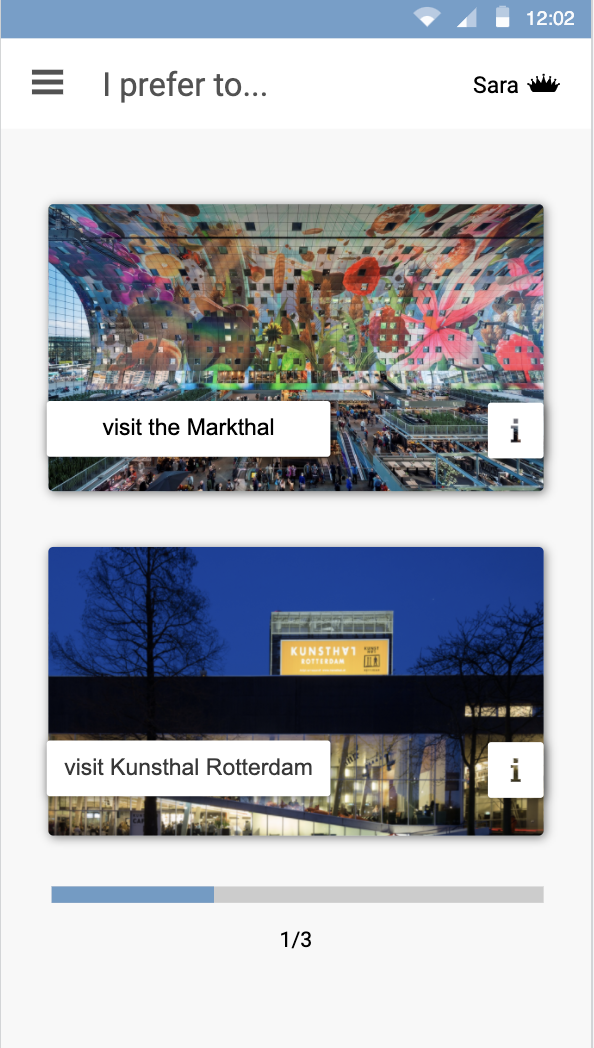
\includegraphics[width=0.3\textwidth]{paper/imgs/hifi_prototypes/pairwise1.png} }}%
    \qquad
    \subfloat[\centering]{{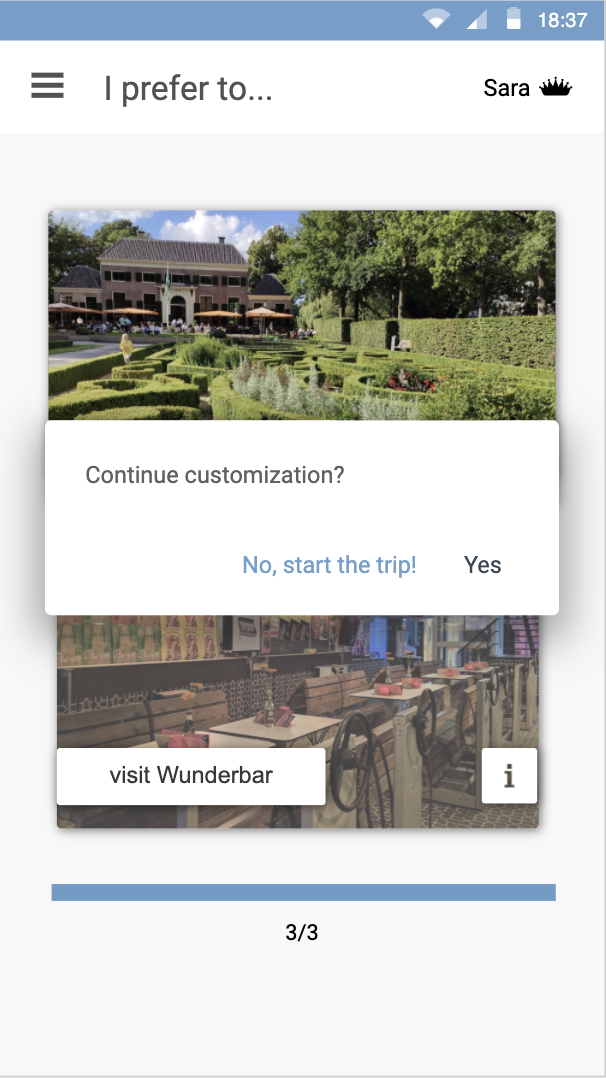
\includegraphics[width=0.3\textwidth]{paper/imgs/hifi_prototypes/pairwise2.png} }}%
    \caption{The pairwise comparison screens }%
    \label{fig:pairwise_comparison_screens}%
\end{figure}

At this point, he can also get additional information about the place, before he selects it. This information is some description of the place, opening times, and contact details as shown in figure \ref{fig:info_screens}.

\begin{figure}[H]
    \centering
    \subfloat[\centering short description]{{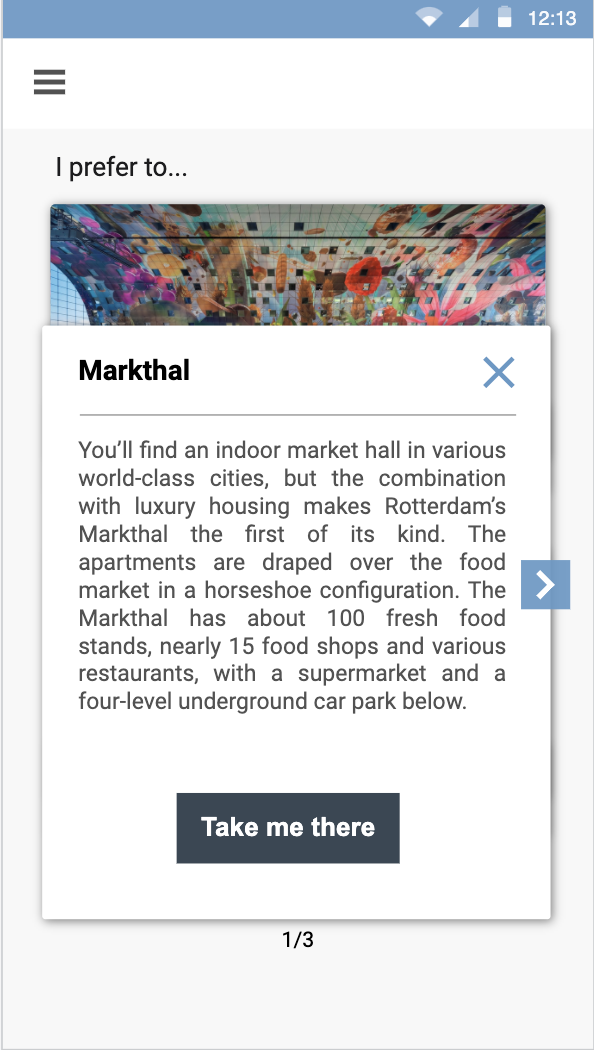
\includegraphics[width=0.25\textwidth]{paper/imgs/hifi_prototypes/info1.png} }}%
    \qquad
    \subfloat[\centering opening hours]{{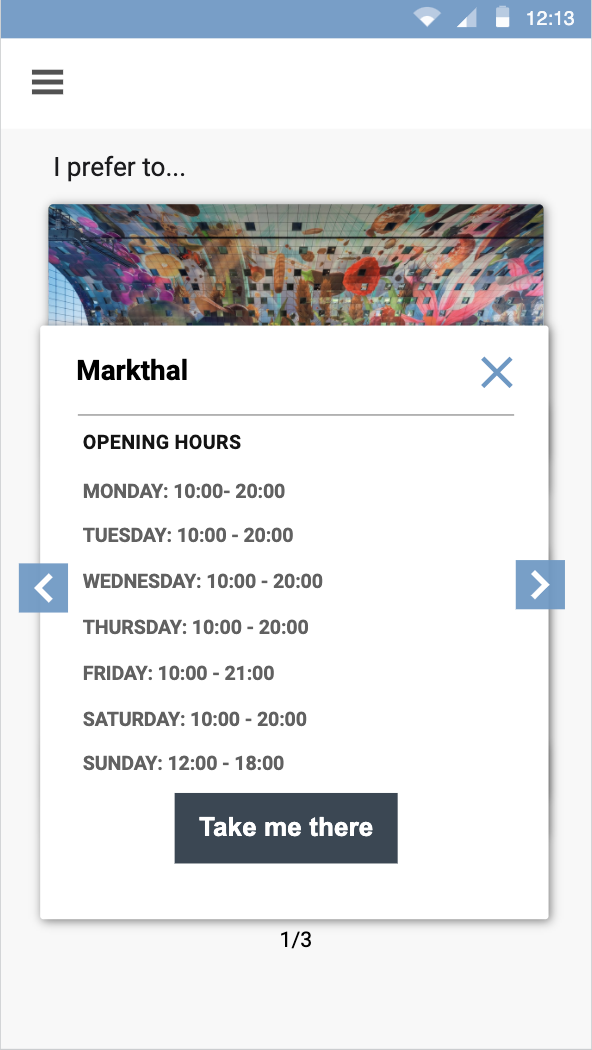
\includegraphics[width=0.25\textwidth]{paper/imgs/hifi_prototypes/info2.png} }}%
    \qquad
    \subfloat[\centering contact details]{{
\includegraphics[width=0.25\textwidth]{paper/imgs/hifi_prototypes/info3.png} }}%
    \caption{The pairwise comparison screens }%
    \label{fig:info_screens}%
\end{figure}

Once the user finishes with the customization, he is shown the results screen with suggested activities as in figure \ref{fig:results_screen}. At this stage, as an administrator, he can select to do all the activities on the list by tapping on “suggest visiting plan” or start from one specific location. 

\begin{figure}[H]
    \centering
    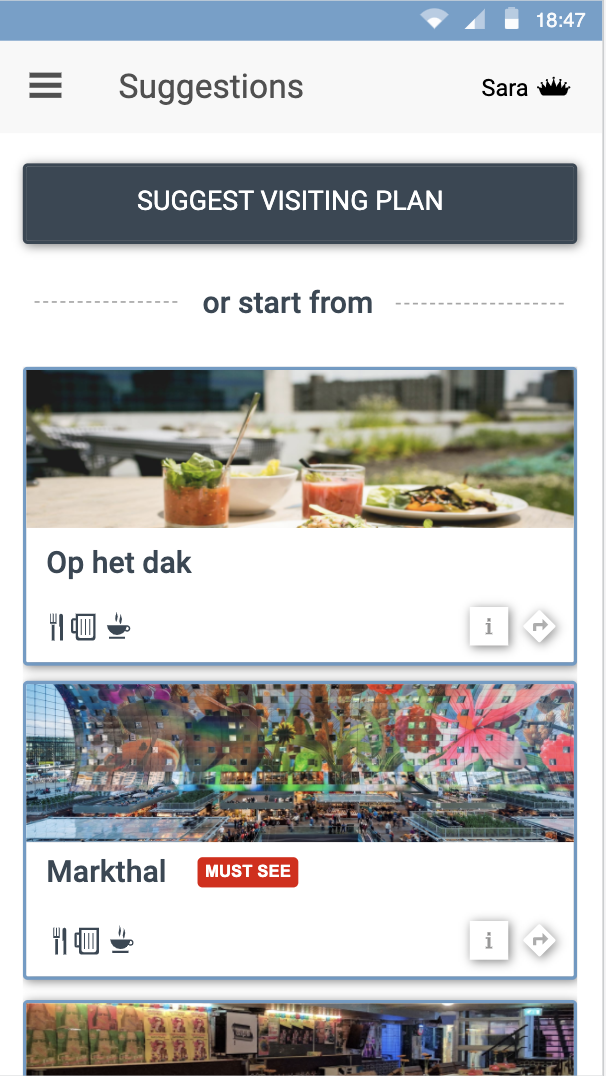
\includegraphics[width=0.3\textwidth]{paper/imgs/hifi_prototypes/results.png}
    \caption{The suggested activities screen}
    \label{fig:results_screen}
\end{figure}

The other users then receive a push notification with the starting point, and they can accept it or reject it (figure \ref{fig:notification_yes_no}).

\begin{figure}[H]
    \centering
    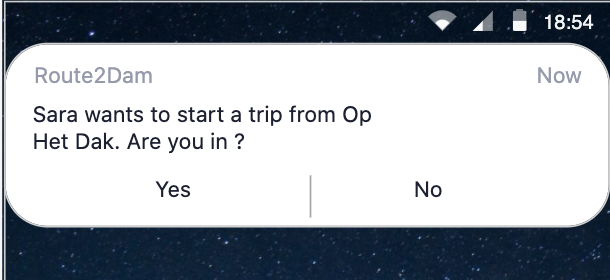
\includegraphics[width=0.3\textwidth]{paper/imgs/hifi_prototypes/push_notification_yes-no.png}
    \caption{The push notification of a suggested activity}
    \label{fig:notification_yes_no}
\end{figure}

Once the starting point is agreed, the option is greyed out (figure \ref{fig:grey_result}). Users can get additional information from the ‘i’ icon or click to the directions icon that will open an external application to navigate them there such as Google maps.

\begin{figure}[H]
    \centering
    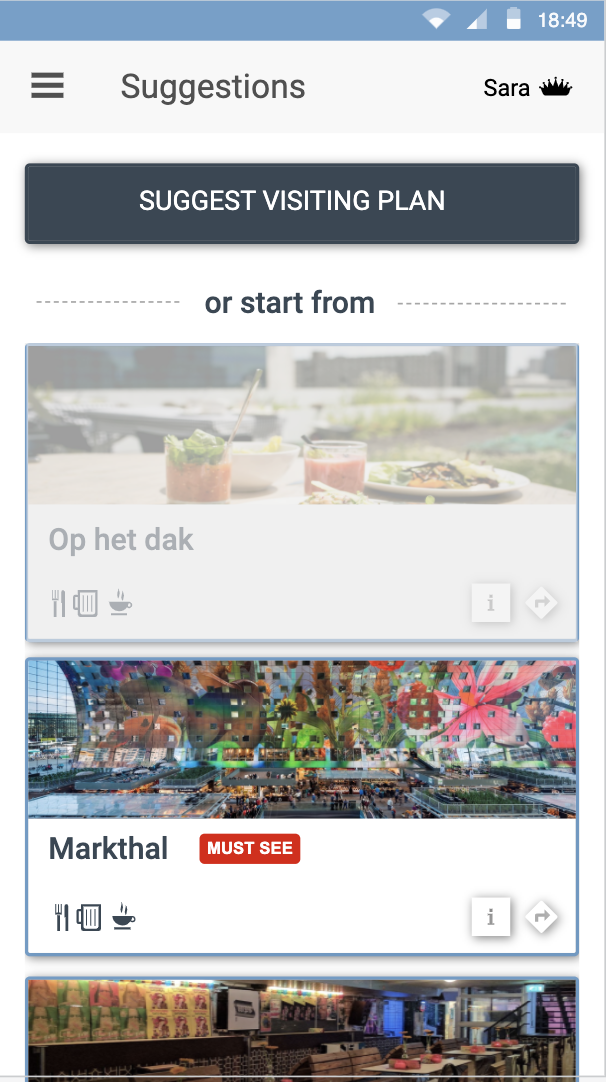
\includegraphics[width=0.3\textwidth]{paper/imgs/hifi_prototypes/results_grey.png}
    \caption{The selected activity is greyed out}
    \label{fig:grey_result}
\end{figure}

Lastly, as it can be seen in figure \ref{fig:must_see} the application can send push notifications throughout the whole time, notifying the users about must-see attractions.

\begin{figure}[H]
    \centering
    
\includegraphics[width=0.3\textwidth]{paper/imgs/hifi_prototypes/push_notification_must_see.png}
    \caption{The 'must-see' push notification}
    \label{fig:must_see}
\end{figure}

\section{Implementation}
Most of the descriptions so far have been mostly conceptually or visually informed. However, in order to get a hollistic understanding of our application, we need to provide more intel behind certain processes and formulas.

\subsection{System Design}

\begin{figure}[H]
    \centering
    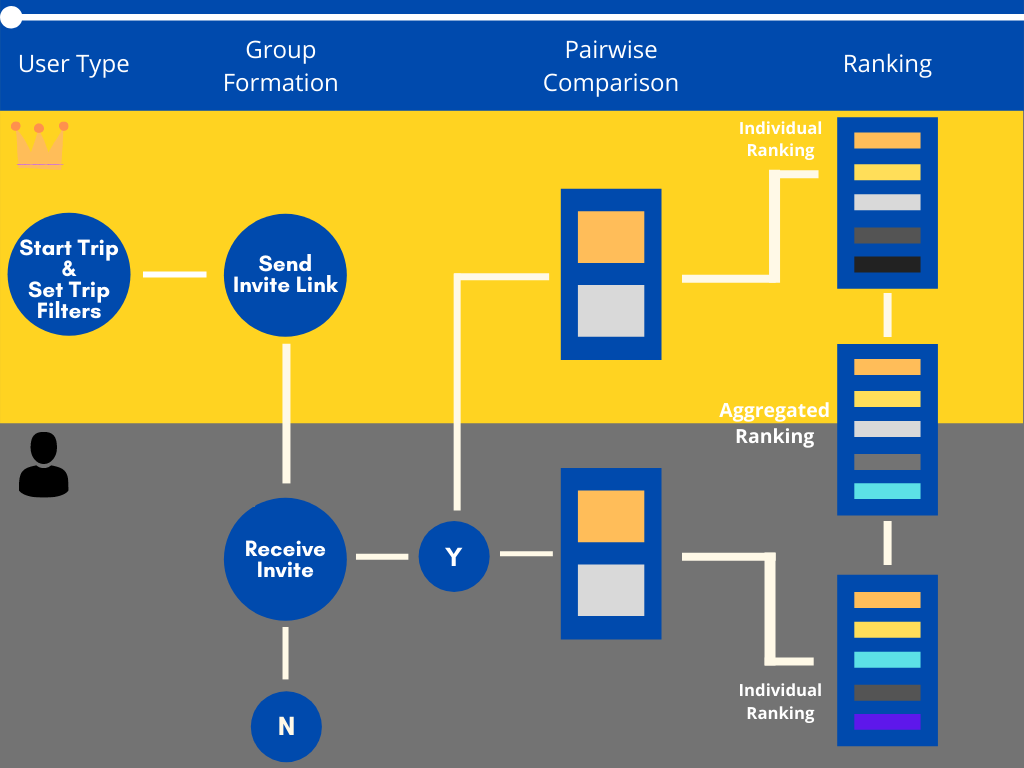
\includegraphics[width=0.95\textwidth]{paper/imgs/flowchart/1.png}
    \caption{First part}
    \label{fig:flowchart1}
\end{figure}

\begin{figure}[H]
    \centering
    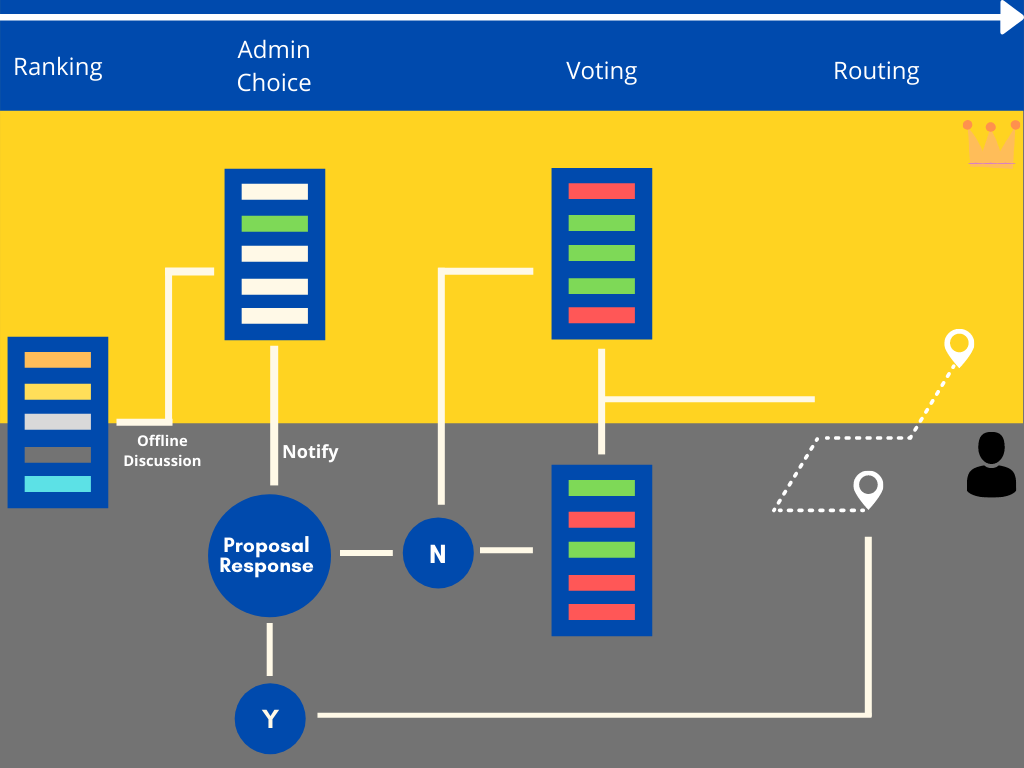
\includegraphics[width=0.95\textwidth]{paper/imgs/flowchart/2.png}
    \caption{Second part}
    \label{fig:flowchart2}
\end{figure}

\subsection{Content and User representation}
A very important part of every model-based system is the representation of real-world objects within the system. For our purpose, we need to clarify the representation of users and activities in our system. As mentioned prior, both objects are represented as vectors. In the case of users $U = {u_1, u_2, \ldots, u_n} $ with being a vector $u \in \mathbb{R}^d$. $d$ refers to the dimensionality corresponding with the user's characteristics. Namely, cultural background, visiting history, budget and activity type preference. Cultural background is a categorical and will be represented as dichotomous variable being either 0 for International or 1 for Dutch. Similar holds for visiting history as we only track whether the user has visited Rotterdam at least once (as 1) or never (as 0). Budget is a ratio variable starting from 0 to $+\inf$, but it will be normalized across all users of the system. The activity type preference is a nominal variable ranging over the taxonomy of attraction groups and restaurant subcategories established by tripadvisor (http://developer-tripadvisor.com/content-api/business-content/categories-subcategories-and-types/). This results in 23 categories that can characterize the attraction preference of a user for a certain type of attraction. Each category leads to a corresponding dimension which can range over \mathbb{N}. Each dimension will track the count for which a user preferred a certain activity type by choosing an item in the pairwise-comparison process. 
To get a better understandin, it is important to understand that we use the same 23 categories to represent an item for the recommender model established in section XXX. The only difference here is that each dimension is a dichotomous variable and every item can belong to $m$ categories. The following XXX illustrates the representation of both a user and an item.

\subsection{Pairwise-comparison model computation}
Given the set of users $U$, items $A$ and a dataset of pairwise comparisons $O$, we can now compute the preference models. For that purpose we have to specify a covariance function $k$, which captures the distance between items and users. Any Mercer-kernel function can be used, but as \citeauthor{guo_GaussianProcessPreference_2010} showed, the standard RBF-kernel suffices. The equation follows 

\begin{equation}
k(x, x') = \exp\left(-\frac{|| x - x' ||^2}{2\sigma^2}\right)
\end{equation}

where $\sigma$ is a hyperparameter that needs to be tuned with hyperparameter optimization techniques. $x$ and $x'$ are vectors which correspond to two user vectors $u$ or two activity vectors $a$. Knowing this, we can compute the quantities $K^*$ and $\Sigma^*$ of \autoref{eqn:computation} to find $\mu^*$ with \autoref{eqn:preddist}.

\subsection{Graph representation}

\clearpage 
\printbibliography

\clearpage
\Large
\begin{tabularx}{\textwidth}{|X|X|X|X|}
\hline
\multicolumn{3}{|c|}{Group 12 Assessment}    \\ \hline
Name                & Contribution & Signature \\ \hline
\hline
Evangelia Giannikou & 100\%        &           \\ \hline
Sorin Dragan        & 100\%        &           \\ \hline
Mikhail Ternyuk     & 100\%        &           \\ \hline
Olusanmi Hundogan   & 100\%        &           \\ \hline
\end{tabularx}

\end{document}